We were mainly interested in answering two questions:

\begin{enumerate}

  \item how far in the future can our system predict well?

  \item how does the knowledge of the grasped object affect the error?

\end{enumerate}

In order to answer the first question, we have checked how the error
on regression changes as the \emph{blind fraction} $0 \leq B \leq 1$
of the grasp increases from $0.1$ to $0.5$. The blind fraction
indicates what percentage of the grasp, from the contact point
backwards, is hidden to the system. In practice, since the sampling
frequency was $50$Hz and each grasp was stretched to $1$ second, a
sequence of $50 \lceil 1-B \rceil$ samples was fed to the SVM, along
with the desired value as regression target, i.e., the actual
position/orientation/posture of the hand at the time of contact. It
was expected that larger values of $B$ would smoothly lead to larger
errors. Figure \ref{fig:B_example} shows a typical situation.

\begin{figure}[htbp]
  \begin{center}
    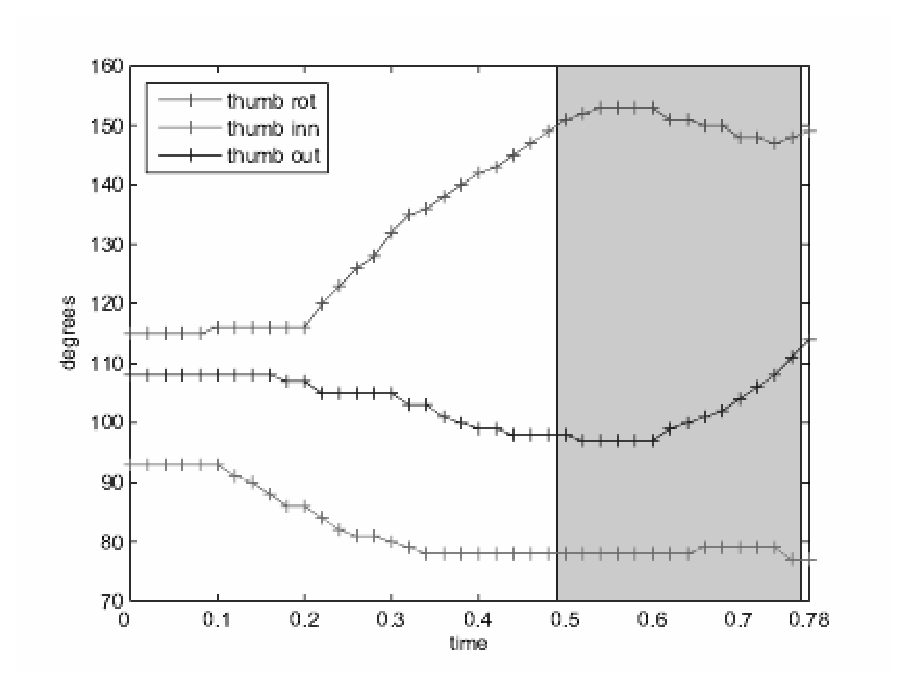
\includegraphics[width=0.5\linewidth]{B_example.eps}
    \caption{The blind window (the grey zone in the Figure) indicates
    what fraction of each grasp, from the contact point backwards, is
    hidden from the system. The data shown is a typical trajectory of
    the thumb (rotation, inner phalanx, outer phalanx) during a
    grasp. In this case the grasp lasts $0.78$ seconds and
    $B=0.375$. The last sample (for $t=0.78$) is the target value and
    is shown to the system in the training phase.}
    \label{fig:B_example}
  \end{center}
\end{figure}

This procedure was repeated independently for each single sensor. The
errors for each sensor were then grouped and averaged accordingly to
their measurement unit and/or meaning: the position of the hand ($3$
sensors, the $x,y,z$ from the FoB), the hand orientation ($3$ sensors,
the azimuth, elevation and roll form the FoB), and the posture of the
hand ($22$ sensors, the joint positions from the
CyberGlove). According to the device resolutions detailed in the
previous Section, we set the $\epsilon$ value related to the SVM
\cite{SmolaTut2004} to $0.1$ inches for the hand position, $0.5$
degrees for the hand orientation and $1$ degree for the hand posture.

In order to answer the second question, we first compared the error
obtained as described above using all sessions for each single object,
so to obtain an estimate of how complex it is to approximate the grasp
for the can, roll and mug, unbiased by the differences among the
subjects. Subsequently we averaged these three errors and compared the
average with the overall error, obtained by joining \emph{all}
sessions together. Figure \ref{fig:err_all} shows the experimental
results.

\begin{figure}[htbp]
  \begin{center}
    \begin{tabular}{cc}
      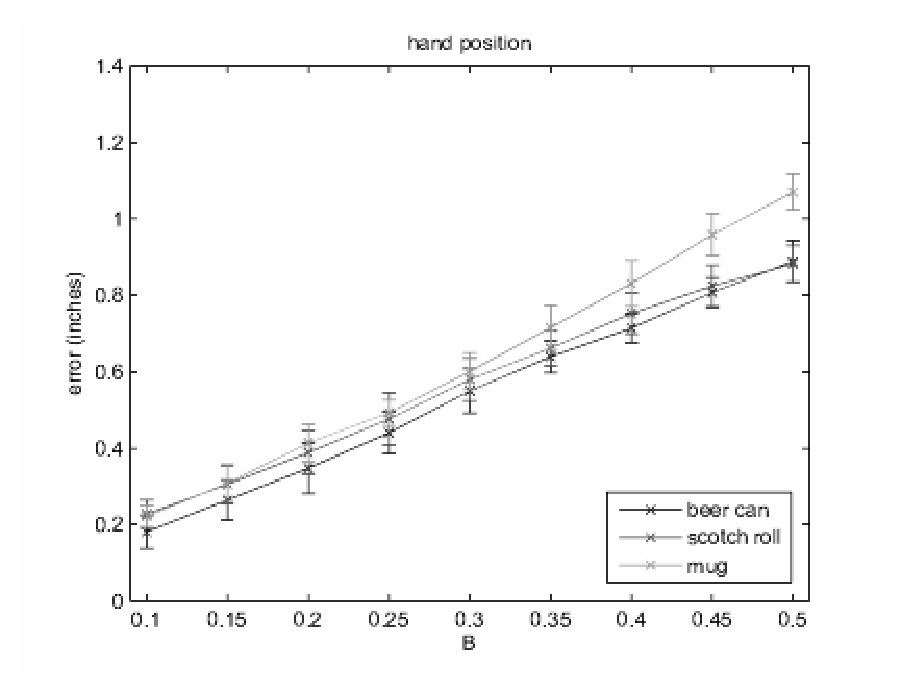
\includegraphics[width=0.45\textwidth]{error_pos.eps} &
      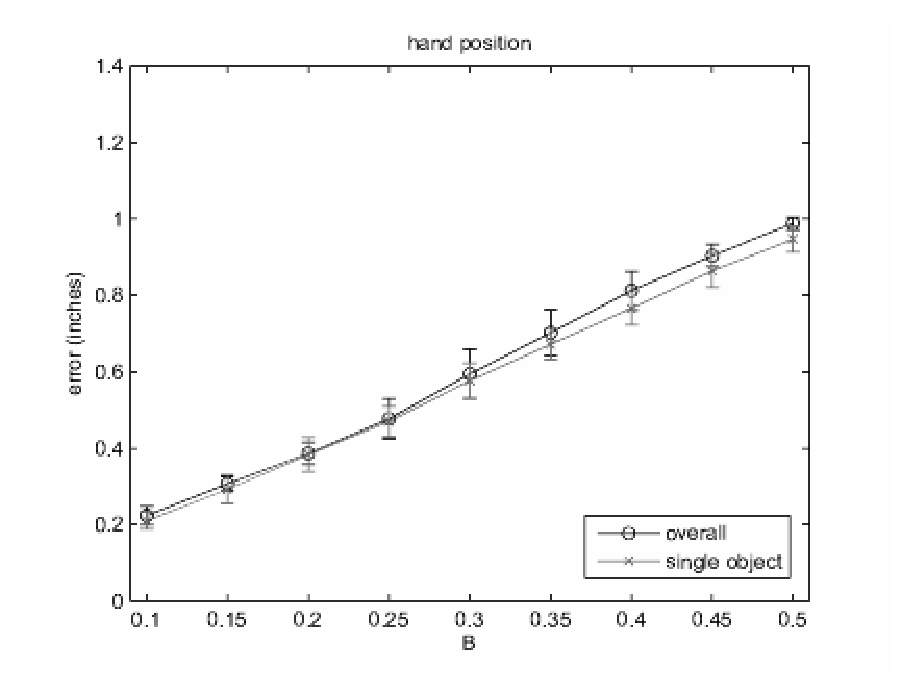
\includegraphics[width=0.45\textwidth]{error_cmp_pos.eps} \\
      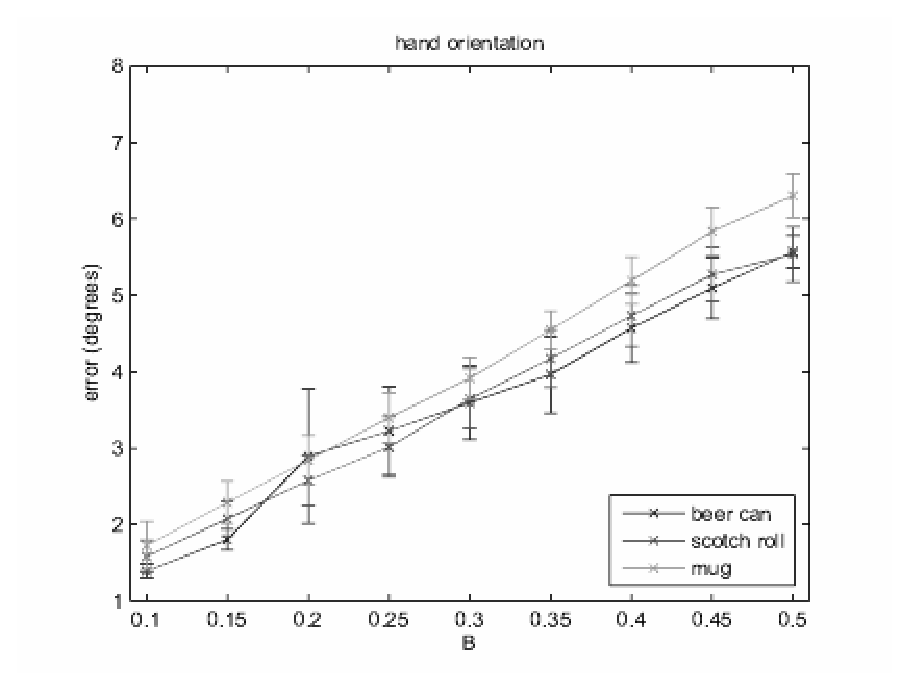
\includegraphics[width=0.45\textwidth]{error_ori.eps} &
      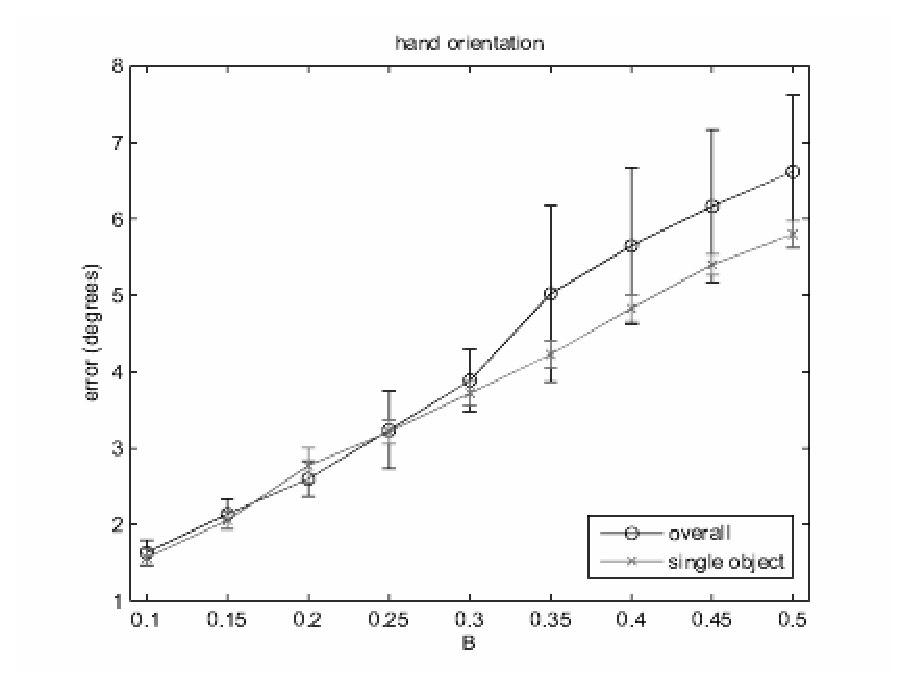
\includegraphics[width=0.45\textwidth]{error_cmp_ori.eps} \\
      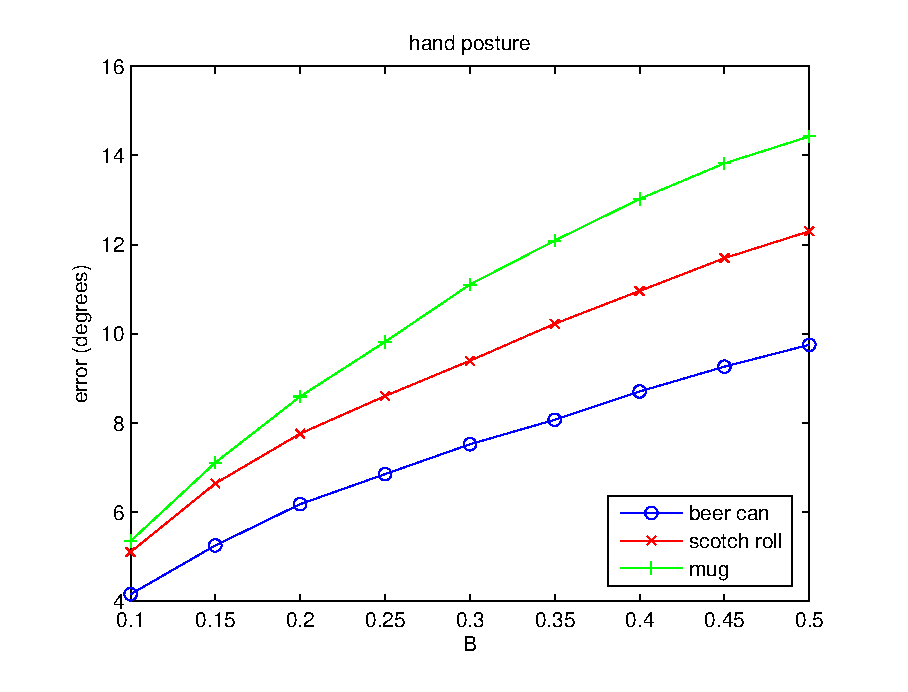
\includegraphics[width=0.45\textwidth]{error_pst.eps} &
      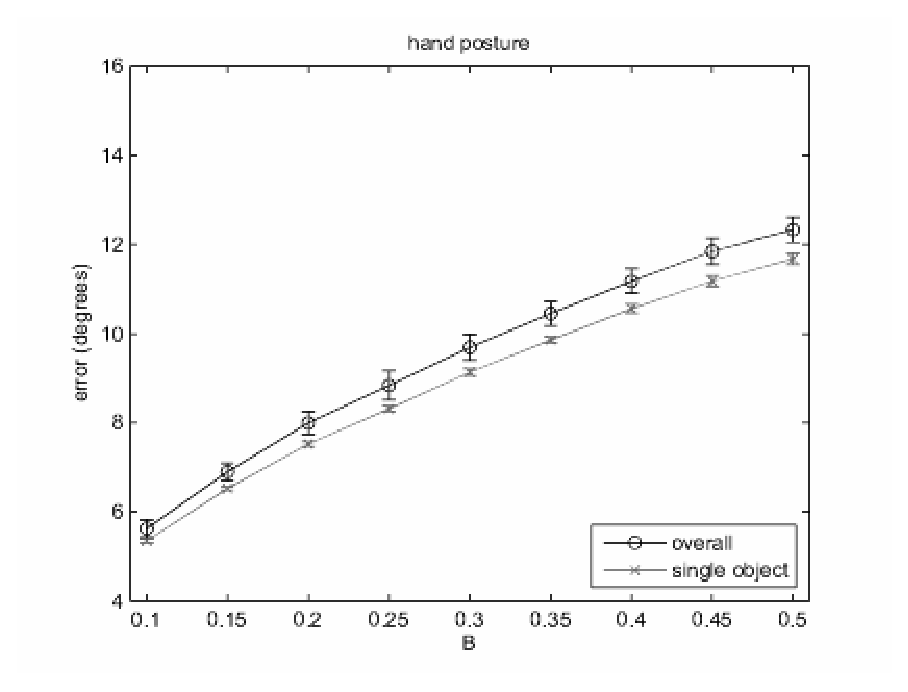
\includegraphics[width=0.45\textwidth]{error_cmp_pst.eps} \\
    \end{tabular}
    \caption{Regression results as the blind fraction $B$ increases
    from $0.1$ to $0.5$. In each row, representing a different set of
    sensors (in turn, hand position, orientation and posture), the
    left-hand side pictures compare the errors on different objects,
    while the right-hand side pictures comapre the average error on
    single objects and the overall error.}
    \label{fig:err_all}
  \end{center}
\end{figure}
